% =============================================================================
% Section 6.1: Faced Challenges
% =============================================================================

\section{Faced Challenges}
\label{sec:challenges}

This section documents the ten most significant technical challenges encountered during the design and implementation of NexaLearn, along with the solutions that were devised. Each challenge is presented as a self-contained case study.

\subsection{Dual-Write Problem in Event Publishing}

\textbf{Challenge.} Many business operations require atomically persisting domain state and publishing an event. For example, when a payment succeeds, the system must both update the \texttt{PaymentIntent} record and notify the Enrollment module. A naive implementation---save to database, then publish event---suffers from the dual-write problem: if the process crashes between the two writes, the event is lost and the enrollment is never activated.

\textbf{Solution.} The transactional outbox pattern described in Section~\ref{sec:event-driven-outbox} solves this by writing the event into an \texttt{OutboxEvent} table within the same database transaction as the business operation. A background poller reads unprocessed events and dispatches them to the appropriate handlers. This guarantees at-least-once delivery without requiring a distributed transaction or a message broker.

\begin{lstlisting}[caption=Outbox event written atomically with business data,label=lst:outbox-tx]
await this.prisma.$transaction(async (tx) => {
  await tx.paymentIntent.update({
    where: { id: paymentIntentId },
    data: { status: PaymentIntentStatus.SUCCEEDED },
  });
  await tx.outboxEvent.create({
    data: {
      aggregateType: 'PaymentIntent',
      aggregateId: paymentIntentId,
      eventType: 'PaymentSucceeded',
      payload: { paymentIntentId, amount, courseId },
    },
  });
});
\end{lstlisting}

\subsection{BigInt Serialisation in JSON}

\textbf{Challenge.} Prisma's auto-generated ID fields use the \texttt{BigInt} type for certain tables with high write throughput. JavaScript's \texttt{JSON.stringify()} does not handle \texttt{BigInt} values, throwing \texttt{TypeError: Do not know how to serialize a BigInt}. This caused silent failures in API responses and webhook payload serialisation.

\textbf{Solution.} A custom \texttt{BigIntSerializer} interceptor was added to the NestJS global serialisation pipeline. The interceptor recursively walks the response object, converts \texttt{BigInt} values to strings (preserving precision), and attaches a custom header \texttt{X-BigInt-Serialized: true} to inform clients. For incoming requests, a custom pipe attempts to parse known ID fields as \texttt{BigInt} where the schema declares them as \texttt{BigInt}.

\begin{lstlisting}[caption=BigInt serialisation interceptor,label=lst:bigint-serializer]
@Injectable()
export class BigIntSerializerInterceptor implements NestInterceptor {
  intercept(context: ExecutionContext, next: CallHandler): Observable<any> {
    return next.handle().pipe(
      map((data) => {
        const serialized = JSON.parse(
          JSON.stringify(data, (_key, value) =>
            typeof value === 'bigint' ? value.toString() : value
          )
        );
        const response = context.switchToHttp().getResponse();
        response.header('X-BigInt-Serialized', 'true');
        return serialized;
      })
    );
  }
}
\end{lstlisting}

\subsection{Optimistic Concurrency Conflicts in Course Mutations}

\textbf{Challenge.} Course editing is a collaborative operation: instructors add modules, rearrange lessons, and update metadata concurrently. Without locking, two simultaneous saves can overwrite each other's changes (lost-update problem). Pessimistic locking was deemed too expensive for a read-heavy workload.

\textbf{Solution.} A \texttt{version} field was added to the \texttt{Course} aggregate. Every update includes \texttt{WHERE version = :currentVersion} in the SQL query. If the version does not match (another request updated the course first), the database returns zero affected rows and the application retries the operation after re-fetching the aggregate. A generic \texttt{withOptimisticRetry()} utility encapsulates this pattern.

\begin{lstlisting}[caption=Optimistic concurrency retry utility,label=lst:optimistic-retry]
async function withOptimisticRetry<T>(
  operation: () => Promise<T>,
  maxRetries = 3
): Promise<T> {
  for (let attempt = 1; attempt <= maxRetries; attempt++) {
    try {
      return await operation();
    } catch (err) {
      if (err instanceof Prisma.PrismaClientKnownRequestError
          && err.code === 'P2025'  // Record not found (version mismatch)
          && attempt < maxRetries) {
        continue;
      }
      throw err;
    }
  }
  throw new ConcurrencyConflictException('Max retries exceeded');
}
\end{lstlisting}

\subsection{AI Pipeline Callback Idempotency}

\textbf{Challenge.} The AI pipeline (Whisper transcription, LLM quiz generation) delivers results via HTTP callbacks. Network retries can cause the same callback payload to arrive multiple times. Without idempotency guarantees, duplicate callbacks could create duplicate transcripts, over-grade quizzes, or trigger duplicate notifications.

\textbf{Solution.} A \texttt{ProjectionEventLedger} table records every successfully processed callback as a row keyed by \texttt{(eventId, handlerName)}. Before processing any callback, the handler attempts to insert a row into the ledger table. If the insert violates the unique constraint (duplicate), the callback is silently acknowledged as already processed. This pattern, known as "insert-else-ignore idempotency," is the same strategy used by Stripe for webhook delivery.

\begin{lstlisting}[caption={Projection event ledger for idempotent callback processing},label=lst:proj-ledger]
async function tryBeginProjectionEvent(
  eventId: string,
  handlerName: string
): Promise<boolean> {
  try {
    await prisma.projectionEventLedger.create({
      data: { eventId, handlerName, status: 'PROCESSING' },
    });
    return true;  // First time — proceed
  } catch (err) {
    if (err.code === 'P2002') return false;  // Duplicate — skip
    throw err;
  }
}
\end{lstlisting}

\subsection{Cross-Bounded-Context Communication Without Tight Coupling}

\textbf{Challenge.} In a DDD-aligned system, each bounded context owns its data. Direct foreign key references between contexts create tight coupling: if the Courses context changes its primary key strategy or shards its database, all contexts referencing its tables must be updated. Early in the project, Prisma schema files across modules referenced each other's IDs directly, creating implicit dependencies.

\textbf{Solution.} Cross-context references use \textbf{value references}: the identifier of an entity in another context is stored as an opaque string rather than a Prisma relation. The referencing context does not import the referenced context's Prisma model; instead, it queries a read-only view or a domain query service provided by the referenced context's interface layer. This enforces the DDD rule that a context may only communicate with another context through its published language (events and query services), never through direct data access.

\subsection{Refresh Token Reuse Detection Under Concurrent Requests}

\textbf{Challenge.} Refresh token rotation invalidates the old token when a new one is issued. If two requests present the same refresh token simultaneously---for example, when a mobile app and a web browser both attempt to refresh at the same instant---the first succeeds but the second fails because the token was already rotated. Worse, a race condition could allow both to succeed if the read--delete--insert cycle is not atomic.

\textbf{Solution.} The Redis session store uses an atomic \texttt{GETDEL} operation (available in Redis 6.2+): the refresh token is retrieved and deleted in a single atomic step. If \texttt{GETDEL} returns null, the token was already consumed. This eliminates the race window entirely.

\begin{lstlisting}[caption=Atomic refresh token consumption,label=lst:redis-getdel]
async function consumeRefreshToken(rawToken: string): Promise<Session | null> {
  const hash = sha256(rawToken);
  const sessionJson = await redis.getdel(`session:${hash}`);
  if (!sessionJson) return null;
  return JSON.parse(sessionJson);
}
\end{lstlisting}

\subsection{Stripe Webhook Exactly-Once Processing}

\textbf{Challenge.} Stripe's webhook delivery guarantees are at-least-once; a single payment event may be delivered multiple times, especially after network interruptions or during Stripe's internal retry window. Without deduplication, duplicate \texttt{payment\_intent.succeeded} events would create multiple enrollment records (already partially addressed by the projection event ledger, but the enrollment creation itself also needed protection).

\textbf{Solution.} The webhook handler wraps enrollment creation in the \texttt{tryBeginProjectionEvent()} pattern from Section~\ref{sec:challenges}. Additionally, the \texttt{PaymentIntent} aggregate enforces a state machine invariant: a payment intent in \texttt{SUCCEEDED} state cannot transition to \texttt{SUCCEEDED} again. This double layer of protection---database-level idempotency and domain-level state machine---ensures that duplicate webhooks cannot produce incorrect state.

\subsection{Video MP4 Rendition Timing}

\textbf{Challenge.} When a video is uploaded to Mux, the asset transitions through several states: \texttt{uploaded} $\rightarrow$ \texttt{ready} $\rightarrow$ \texttt{mp4\_rendition\_ready}. The AI pipeline requires an MP4 download URL to extract audio for Whisper transcription, but the MP4 rendition becomes available asynchronously---typically 10--60 seconds after \texttt{asset.ready}. Polling for the MP4 URL introduced unpredictable latency.

\textbf{Solution.} A two-stage state machine was added to the \texttt{VideoAsset} aggregate. The asset transitions to \texttt{READY} when the HLS stream is available, then separately transitions to \texttt{MP4\_AVAILABLE} when Mux fires the \texttt{video.asset.mp4\_rendition.ready} webhook. The AI pipeline is triggered only when the asset reaches \texttt{MP4\_AVAILABLE}. This cleanly separates playback readiness from AI-readiness.

\begin{figure}[H]
  \centering
  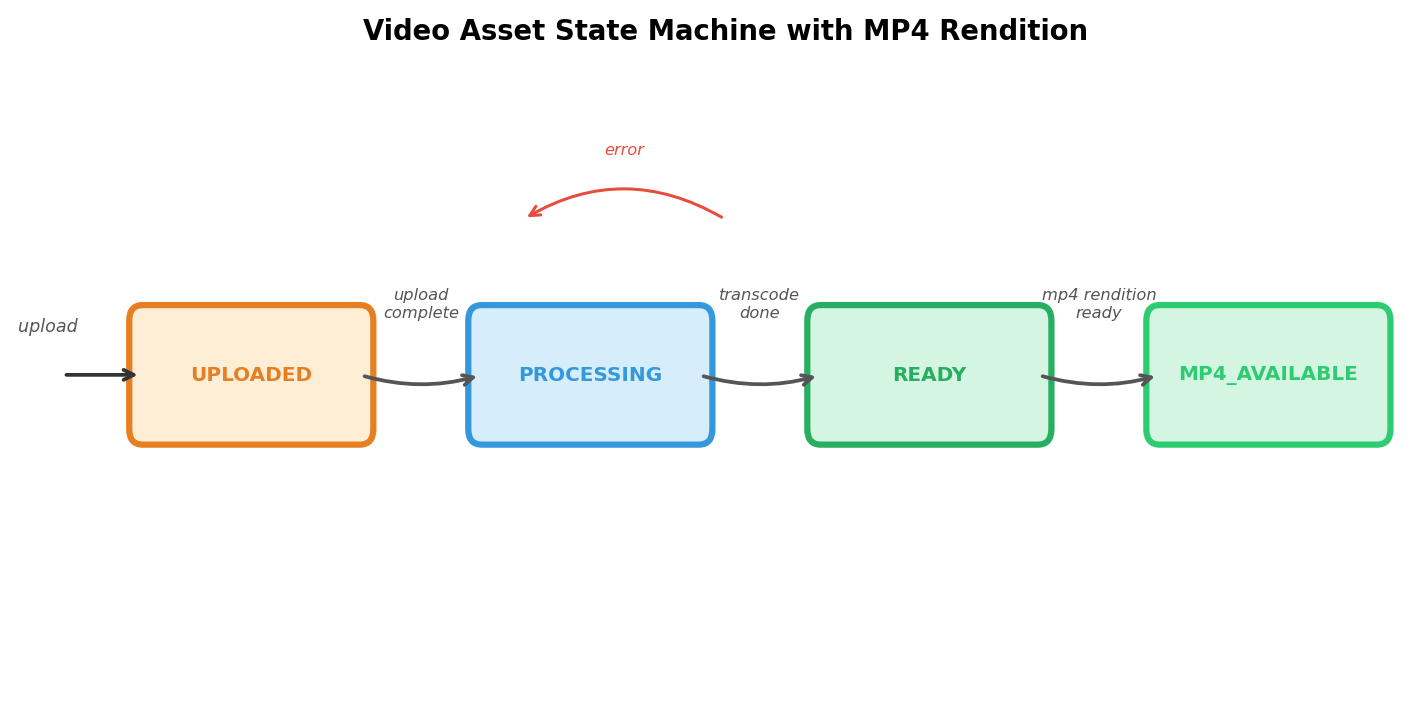
\includegraphics[width=0.6\textwidth]{images/video_rendition_statemachine.png}
  \caption{Video Asset State Machine with MP4 Rendition Tracking}\label{fig:video-rendition-statemachine}
\end{figure}

\subsection{Rate Limiting State Across Multiple Instances}

\textbf{Challenge.} The default NestJS throttler module stores rate-limit counters in memory. When the application is scaled to multiple instances (horizontal scaling), each instance maintains its own counter, allowing a client to exceed the global rate limit by distributing requests across instances.

\textbf{Solution.} The Throttler module was configured with \texttt{ThrottlerStorageRedisService}, which stores rate-limit counters in Redis. All instances share the same Redis-backed counter, enforcing a global rate limit irrespective of which instance processes the request. The TTL of the Redis key matches the rate-limit window duration.

\subsection{Complex Quiz Grading with Async Short-Answer Questions}

\textbf{Challenge.} Quizzes can contain short-answer questions that require AI grading via the LLM pipeline. Unlike multiple-choice questions (graded synchronously), short-answer grading is asynchronous: the answer is submitted, an \texttt{ShortAnswerGradeRequestedEvent} is published, and the grade arrives via a webhook callback. This introduces a partial grading state where some questions are scored and others are pending.

\textbf{Solution.} The \texttt{QuizAttempt} aggregate tracks per-question grading status through a \texttt{GradingStatus} enum (\texttt{PENDING}, \texttt{AUTO\_GRADED}, \texttt{AI\_GRADED}, \texttt{REVIEW\_REQUIRED}). When all questions reach a final status, the aggregate computes the total score and transitions to \texttt{GRADED}. If any question remains in \texttt{PENDING} beyond a configurable timeout (30 minutes), the aggregate escalates to \texttt{REVIEW\_REQUIRED} for manual instructor intervention.
